%===========================================================================================
% TEMPLATE FOR STANDARD EXAM
% (with some sample problem types)
% Original by Laura
% Modified by Justin Watson
%===========================================================================================
\documentclass[11pt,epsfig]{article}

\usepackage{amsmath,amssymb}   % Provies math symbols 
\usepackage{mathtools}         % Tools for mathematical typesetting 
\usepackage{graphics}          % Inclusion of graphics in LaTex documents
\usepackage{graphicx}          % Extensions to graphics
\usepackage{scrextend}         % Adds ability to change margin on a block of text.
\usepackage{etoolbox}          % Adds programming facilities 
\usepackage{mhchem}            % Adds ability to correctly write chemical reactions
\usepackage{enumitem}          % Controls layout of itemize, enumerate, etc.

%===========================================================================================
% Create logical variables to turn on or off solutions and graphics elements
%===========================================================================================

\providetoggle{Solution}
\settoggle{Solution}{false}    % false = do not typeset solution; true = typeset solution 

\providetoggle{NoFig}
\settoggle{NoFig}{true}        % true = inlcude graphics; false = do not include graphics

\oddsidemargin=0in
\evensidemargin=0in
\textwidth=6.3in
\topmargin=-.5in
\textheight=9in

\parindent=0in
\pagestyle{empty}



%------------------------------------------------------------------
% PROBLEM, PART, AND POINT COUNTING...

% Create the problem number counter.  Initialize to zero.
\newcounter{problemnum}

% Specify that problems should be labeled with arabic numerals.
\renewcommand{\theproblemnum}{\arabic{problemnum}}


% Create the part-within-a-problem counter, "within" the problem counter.
% This counter resets to zero automatically every time the PROBLEMNUM counter
% is incremented.
\newcounter{partnum}[problemnum]

% Specify that parts should be labeled with lowercase letters.
\renewcommand{\thepartnum}{\alph{partnum}}

% Make a counter to keep track of total points assigned to problems...
\newcounter{totalpoints}

% Make counters to keep track of points for parts...
\newcounter{curprobpts}		% Points assigned for the problem as a whole.
\newcounter{totalparts}		% Total points assigned to the various parts.

% Make a counter to keep track of the number of points on each page...
\newcounter{pagepoints}
% This counter is reset each time a page is printed.

% This "program" keeps track of how many points appear on each page, so that
% the total can be printed on the page itself.  Points are added to the total
% for a page when the PART (not the problem) they are assigned to is specified.
% When a problem without parts appears, the PAGEPOINTS are incremented directly
% from the problem as a whole (CURPROBPTS).


%---------------------------------------------------------------------------


% The \problem environment first checks the information about the previous
% problem.  If no parts appeared (or if they were all assigned zero points,
% then it increments TOTALPOINTS directly from CURPROBPTS, the points assigned
% to the last problem as a whole.  If the last problem did contain parts, it
% checks to make sure that their point values total up to the correct sum.
% It then puts the problem number on the page, along with the points assigned
% to it.

\newenvironment{problem}[1]{
% STATEMENTS TO BE EXECUTED WHEN A NEW PROBLEM IS BEGUN:
%
% Increment the problem number counter, and set the current \ref value to that
% number.
\refstepcounter{problemnum}
%
% Add some vspace to separate from the last problem.
\vspace{0.15in} \par
%
\setcounter{curprobpts}{#1} \setcounter{totalparts}{0}	% Reset counters.
%
% Now put in the "announcement" on the page.
{\Large \bf \theproblemnum. \normalsize ({\it \arabic{curprobpts} point\null\ifnum \value{curprobpts} = 1\else s\fi}\/)}
}{
% STATEMENTS TO BE EXECUTED WHEN AN OLD PROBLEM IS ENDED:
%
% If no parts to problem, then increment TOTALPOINTS and PAGEPOINTS for the
% entire problem at once.
\ifnum \value{totalparts} = 0
	\addtocounter{totalpoints}{\value{curprobpts}}	% Add pts to total.
	\addtocounter{pagepoints}{\value{curprobpts}}	% Add pts to page total.
%
% If there were parts for the problem, then check to make sure they total up
% to the same number of points that the problem is worth. Issue a warning
% if not.
\else \ifnum \value{totalparts} = \value{curprobpts}
	\else \typeout{}
	\typeout{!!!!!!!   POINT ACCOUNTING ERROR   !!!!!!!!}
	\typeout{PROBLEM [\theproblemnum] WAS ALLOCATED \arabic{curprobpts} POINTS,}
	\typeout{BUT CONTAINS PARTS TOTALLING \arabic{totalparts} POINTS!}
	\typeout{}
	\fi
\fi
}


%---------------------------------------------------------------------------


% The \newpart command increments the part counter and displays an appropriate
% lowercase letter to mark the part.  It adds points to the point counter
% immediately.  If 0 points are specified, no point announcement is made.
% Otherwise, the announcement is in scriptsize italics.

\newcommand{\newpart}[1]
{
\refstepcounter{partnum}	% Set the current \ref value to the part number.
\hspace{0.25in}		% Indent the part by a quarter inch.
%
% If points are to be printed for this problem (signaled by point value > 0),
% then put them in in scriptsize italics.
\ifnum #1 > 0
	\makebox[0.5in][l]{{\bf \thepartnum.} {\bf ({\it #1 pt\ifnum #1 = 1\else s\fi\/}) \,\,}}
\else
	\makebox[0.25in][l]{({\bf \thepartnum})}
\fi
%
\hspace{0.1in}		% Lead the material away from the part "number".
%
\addtocounter{totalparts}{#1}	% Add points to totalparts for this problem.
\addtocounter{pagepoints}{#1}	% Add points to total for this page.
\addtocounter{totalpoints}{#1}	% Add points to total for entire test.
}


%---------------------------------------------------------------------------



% Just in case you want to skip some numbers in your test...

\newcommand{\skipproblem}[1]{\addtocounter{problemnum}{#1}}



%---------------------------------------------------------------------------


% The \showpoints command simply gives a count of the total points read in up to
% the location at which the command is placed.  Typically, one places one
% \showpoints command at the end of the latex file, just prior to the
% \end{document} command.  It can appear elsewhere, however.

\newcommand{\showpoints}
{
\typeout{}  
\typeout{====> A TOTAL OF \arabic{totalpoints} POINTS WERE READ.}
\typeout{}
}


%---------------------------------------------------------------------------



\begin{document}

\iftoggle{Solution}{
  \settoggle{NoFig}{false}     % This is currently set to show certain graphics when 
}                              % solution is true and others when solution is false.

%===========================================================================================
% Cover Sheet
%===========================================================================================

\centerline{\huge \bf Course Title}         
\vfill
\centerline{\huge \bf Exam 1: Topic}        
\vfill \vfill
   
Class Number and Section                     

MM/DD/YYYY \hfill                           % (date of test)
{\bf Name: } $\underbracket[0.5pt][0pt]{\hspace{2.7in}}_{\mbox{\tiny Please print your name clearly}}$
\vfill \vfill \vfill

{\bf Read all of the following information before starting the exam:}
\vspace{1pc}

\begin{itemize}                             % (change info. as desired)
	\item  Show all work, clearly and in order, if you want to get full credit.  I reserve the right to take off points if I cannot see how you 	arrived at your answer (even if your final answer is correct).
	
	\item Justify your answers algebraically whenever possible to ensure 
	full credit. When you do use your calculator (if a calculator is allowed),
	sketch all relevant graphs and explain all relevant mathematics.
	
	\item  Circle or otherwise indicate your final answers.

	\item  Please keep your written answers brief; be clear and to the point.
	I will take points off for rambling and for incorrect or irrelevant 
	statements.
		
	\item  This test has 10 problems        % (number of problems)
	and is worth 100 points,                % (insert total number of points)  
   partial credit will be given for incomplete answers.  If you are
   not sure how to answer a problem give as much information as you can.	
   It is your responsibility to make sure that you have all of the pages!
	
	\item  You will have 1 hour 50 minutes to complete the exam.  
	
	\item  Good luck!
\end{itemize}

\vfill \vfill \vfill

\clearpage

%===========================================================================================
% Question 1
%===========================================================================================

\begin{problem}{8}
\let\clearpage\relax
Label each of the regions of the following flow regime map.  Clearly label the x and y axis including any units and give the range of  values for each of the flow regimes on the x and y axis.  
\iftoggle{NoFig}{
\begin{center}
         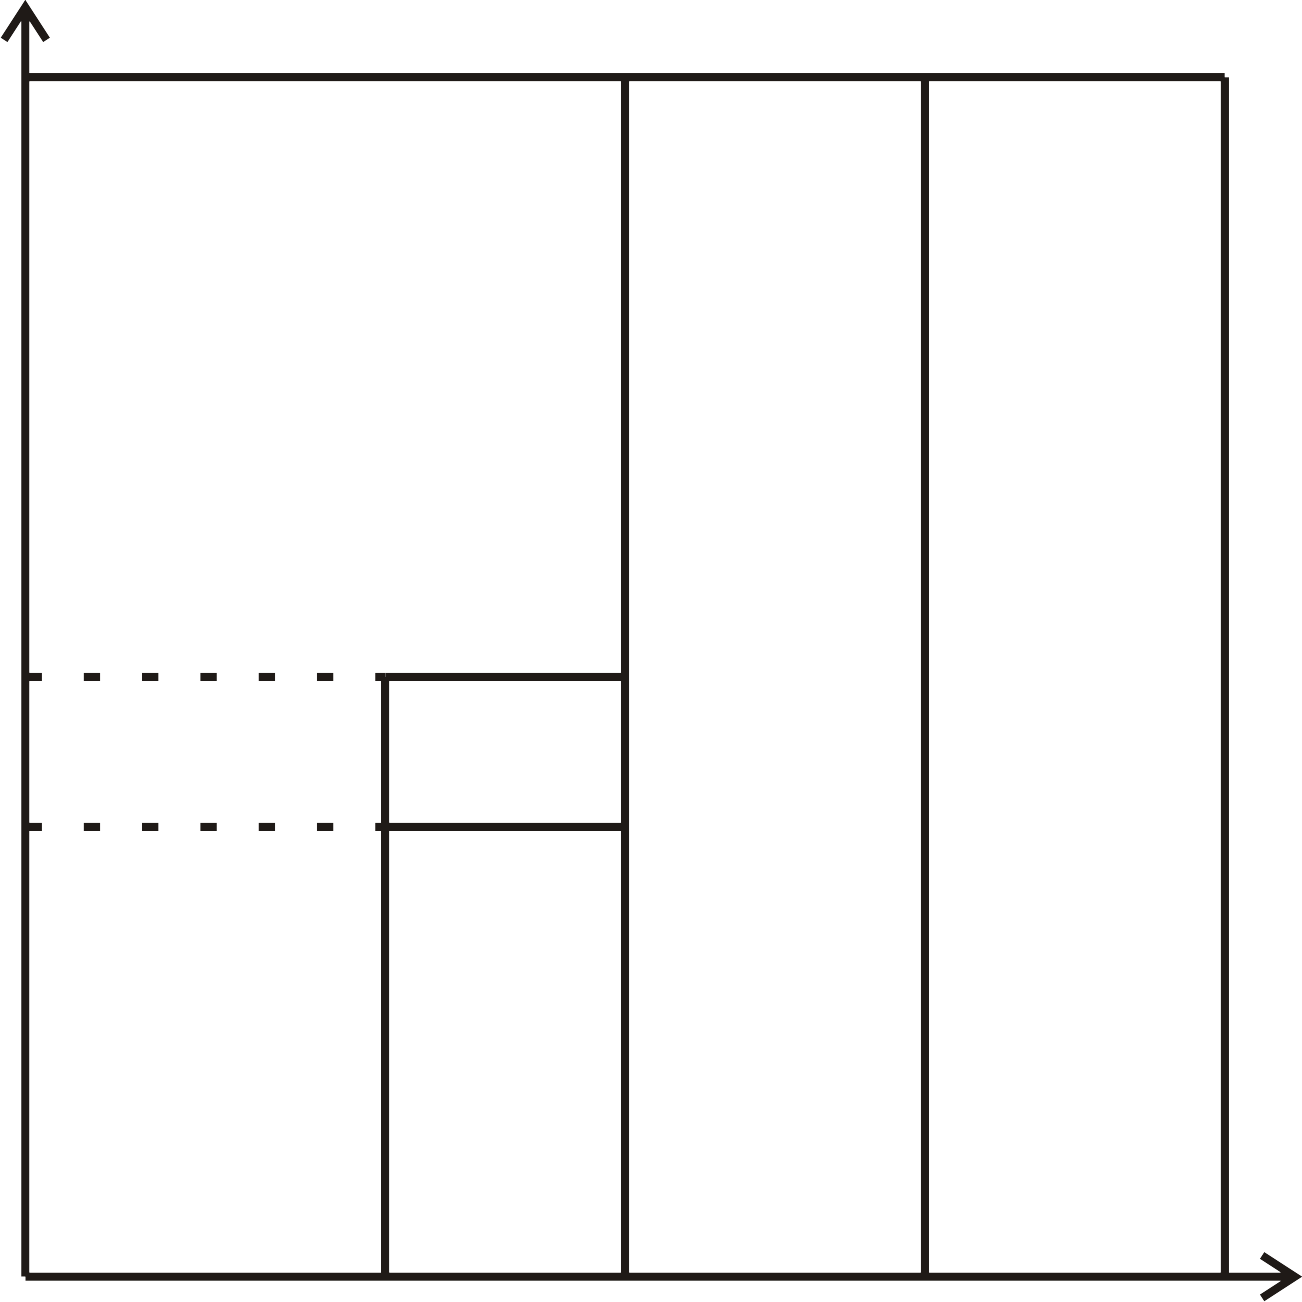
\includegraphics[width=3in]{../Figures/FlowMap.png}
\end{center}
}

%
% Solution
%
\iftoggle{Solution}{
  \vspace{12pt}
  \begin{addmargin}[1em]{2em}
    \textbf{Solution:}
    \vspace{12pt}
\begin{center}
         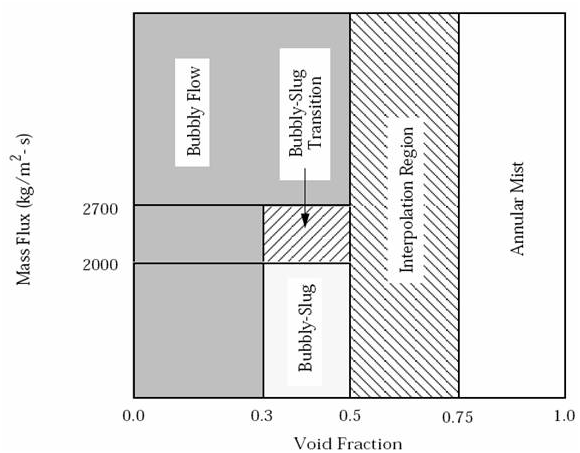
\includegraphics[width=4in]{../Figures/FlowMapSol.png}
\end{center}    
   \end{addmargin}
}


\vfill
\end{problem}

\clearpage

%===========================================================================================
% Question 2
%===========================================================================================

\begin{problem}{8}
\let\clearpage\relax
This problem involves setting up the truncation error analysis for the given fully implicit mass equation with constant positive velocity shown below.

\begin{equation*}
\text{Difference Equation: }\frac{\rho^{n+1}_j-\rho^{n}_j}{\Delta t} + v \frac{\rho^{n+1}_j-\rho^{n+1}_{j-1}}{\Delta x_j} = 0
\end{equation*}

\newpart{2}
 Plot an clearly state the variable that you are making the error evaluation about.  
%
% Solution
%
\iftoggle{Solution}{
  \vspace{12pt}
  \begin{addmargin}[1em]{2em}
    \textbf{Solution:}
    \vspace{12pt}

Use a Taylor series to expand about the point $\rho^{n+1}_j$.  We need one expression for $\rho^{n+1}_{j-1}$ and one for $\rho^n_j$:

\centerline{
  \mbox{
    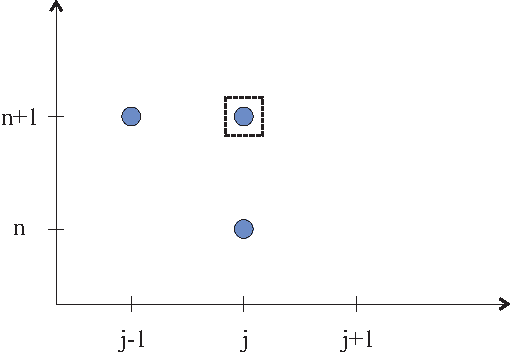
\includegraphics[width=2in]{../Figures/TaylorSol.pdf}
  }
}
   \end{addmargin}
}
\vfill

\newpart{6}
Write the Taylor series expansion for the two remaining variables about the point chosen above. (NOTE: you don't have to do anything beyond writing the Taylor series expansion.)
%
% Solution
%
\iftoggle{Solution}{
  \vspace{12pt}
  \begin{addmargin}[1em]{2em}
    \textbf{Solution:}
    \vspace{12pt}

\begin{equation*}
   \rho^n_j = \rho^{n+1}_j - \frac{\Delta t}{1!} \left.\frac{\partial \rho}{\partial t}\right|^{n+1}_j + \frac{\Delta t^2}{2!} \left.\frac{\partial^2 \rho}{\partial t^2}\right|^{n+1}_j - \frac{\Delta t^3}{3!} \left.\frac{\partial^3 \rho}{\partial t^3}\right|^{n+1}_j + \cdots
\end{equation*}
\begin{equation*}
   \rho^{n+1}_{j-1} = \rho^{n+1}_j - \frac{\Delta x}{1!} \left.\frac{\partial \rho}{\partial x}\right|^{n+1}_j + \frac{\Delta x^2}{2!} \left.\frac{\partial^2 \rho}{\partial x^2}\right|^{n+1}_j - \frac{\Delta x^3}{3!} \left.\frac{\partial^3 \rho}{\partial x^3}\right|^{n+1}_j + \cdots
\end{equation*}

   \end{addmargin}
}

\vfill

\vfill
\end{problem}

\clearpage

%===========================================================================================
% Scrap Page 
%===========================================================================================
% NOTE: The scrap page and equation sheet are not typeset if solution is true.  
\iftoggle{NoFig}{


{\large \bf Scrap Page}

(please do not remove this page from the test packet)
\clearpage

%===========================================================================================
% Equation Sheet
%===========================================================================================
{\large \bf Useful Equations}
\vspace{12pt}

\begin{equation*}
   f(x) = f(x_0) + \left( x - x_0 \right)\left. \frac{ d f }{ d x } \right|_{x=x_0}  + \left( x - x_0 \right)^2\left. \frac{1}{2} \frac{ d^2 f }{ d x^2 } \right|_{x=x_0}  + \cdots
\end{equation*}

\begin{multline*}
   f(x,y) = f(x_0, y_0) +
   \Delta x \left. \frac{ \partial f }{\partial x } \right|_{x_0, y_0} +
   \Delta y \left. \frac{ \partial f }{\partial y } \right|_{x_0, y_0} +
   \Delta x^2 \frac{1}{2} \left. \frac{ \partial^2 f }{\partial x^2 } \right|_{x_0, y_0} +\\
   \Delta x \Delta y \left. \frac{ \partial^2 f }{ \partial x \partial y } \right|_{x_0, y_0} +
   \Delta y^2 \frac{1}{2} \left. \frac{ \partial^2 f }{\partial y^2 } \right|_{x_0, y_0} + \cdots
\end{multline*}

\begin{multline*}
   g(x,y) = g(x_0, y_0) +
   \Delta x \left. \frac{ \partial g }{\partial x } \right|_{x_0, y_0} +
   \Delta y \left. \frac{ \partial g }{\partial y } \right|_{x_0, y_0} +
   \Delta x^2 \frac{1}{2} \left. \frac{ \partial^2 g }{\partial x^2 } \right|_{x_0, y_0} +\\
   \Delta x \Delta y \left. \frac{ \partial^2 g }{ \partial x \partial y } \right|_{x_0, y_0} +
   \Delta y^2 \frac{1}{2} \left. \frac{ \partial^2 g }{\partial y^2 } \right|_{x_0, y_0} + \cdots
\end{multline*}

\begin{equation*}
\frac{\partial \rho}{\partial t}+\nabla\cdot(\rho \vec{v})=0
\end{equation*}

\begin{equation*}
\frac{\partial \rho e}{\partial t}+\nabla\cdot(\rho e\vec{v})+P\nabla\cdot\vec{v}=q_{wl}
\end{equation*}

\begin{equation*}
\frac{\partial \vec{v}}{\partial t}+\vec{v}\nabla\cdot(\vec{v})+\frac{1}{\rho}\nabla P + K\vec{v}^2=0
\end{equation*}

\begin{equation*}
         r = \frac{ h_3 }{ h_2 } = \frac{ h_2 }{ h_1 } 
\end{equation*}

\begin{align*}
   &f_1 = f_{exact} + a h^p_1\\
   &f_2 = f_{exact} + a h^p_2\\
   &f_3 = f_{exact} + a h^p_3
\end{align*}

\begin{equation*}
   \frac{ f_3 - f_2 }{ f_2 - f_1 } = \frac{ h^p_2 }{ h^p_1 } = r^p
\end{equation*}

\begin{equation*}
   p = \frac{ \ln \left( \frac{ f_3 - f_2 }{ f_2 - f_1 } \right) }{ \ln \left( r \right) }
\end{equation*}

\begin{equation*}
   f_{exact} = f_1 - \frac{ f_2 - f_1 }{ r^p - 1 }
\end{equation*}

\begin{equation*}
\frac{1}{2} \rho v^2_1 + P_1 = \frac{1}{2} \rho v^2_2 + P_2 + \Delta P_l
\end{equation*}

\begin{equation*}
\Delta P_l = 
\frac{1}{2} \rho v^2_1 
\left(
1
-\frac{A_1}{A_2}
\right)^2
\end{equation*} 


}

\showpoints
\end{document}


